C++ lambda expressions, also referred to as anonymous function objects, unnamed function objects, closures, or simply lambdas, are a convenient way to express a kernel right where it is used. This section describes how to represent a kernel as a C++ lambda expression. This expands on the introductory refresher on C++ lambda functions, in Chapter 1, which included some coding samples with output.\par

C++ lambda expressions are very powerful and have an expressive syntax, but only a specific subset of the full C++ lambda expression syntax is required (and supported) when expressing a kernel.\par

\hspace*{\fill} \par %插入空行
Figure 10-2. Kernel defined using a lambda expression
\begin{lstlisting}[caption={}]
h.parallel_for(size,
	// This is the start of a kernel lambda expression:
	[=](id<1> i) {
		data_acc[i] = data_acc[i] + 1;
	}
	// This is the end of the kernel lambda expression.
);
\end{lstlisting}

\hspace*{\fill} \par %插入空行
\textbf{Elements of a Kernel Lambda Expression}

Figure 10-2 shows a kernel written as a typical lambda expression—the code examples so far in this book have used this syntax.\par

The illustration in Figure 10-3 shows more elements of a lambda expression that may be used with kernels, but many of these elements are not typical. In most cases, the lambda defaults are sufficient, so a typical kernel lambda expression looks more like the lambda expression in Figure 10-2 than the more complicated lambda expression in Figure 10-3.\par

\hspace*{\fill} \par %插入空行
Figure 10-3. More elements of a kernel lambda expression, including  optional elements
\begin{center}
	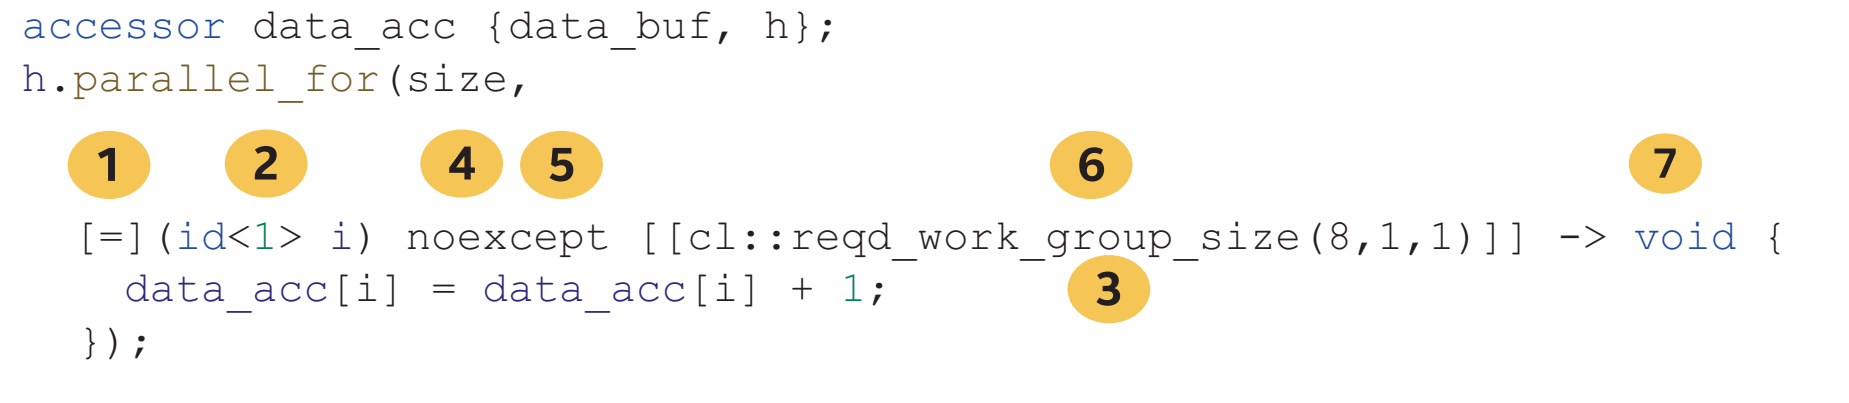
\includegraphics[width=1.0\textwidth]{content/chapter-10/images/2}
\end{center}

\begin{enumerate}
	\item The first part of a lambda expression describes the lambda captures. Capturing a variable from a surrounding scope enables it to be used within the lambda expression, without explicitly passing it to the lambda expression as a parameter.\\
	C++ lambda expressions support capturing a variable by copying it or by creating a reference to it, but for kernel lambda expressions, variables may only be captured by copy. General practice is to simply use the default capture mode [=], which implicitly captures all variables by value, although it is possible to explicitly name each captured variable as well. Any variable used within a kernel that is not captured by value will cause a compile-time error.
	\item The second part of a lambda expression describes parameters that are passed to the lambda expression, just like parameters that are passed to named functions.\\
	For kernel lambda expressions, the parameters depend on how the kernel was invoked and usually identify the index of the work-item in the parallel execution space. Please refer to Chapter 4 for more details about the various parallel execution spaces and how to identify the index of a work-item in each execution space.
	\item The last part of the lambda expression defines the lambda function body. For a kernel lambda expression, the function body describes the operations that should be performed at each index in the parallel execution space.\\
	There are other parts of a lambda expression that are supported for kernels, but are either optional or infrequently used:
	\item Some specifiers (such as mutable) may be supported, but their use is not recommended, and support may be removed in future versions of SYCL (it is gone in the provisional SYCL 2020) or DPC++. None is shown in the example code.
	\item The exception specification is supported, but must be noexcept if provided, since exceptions are not supported for kernels.
	\item Lambda attributes are supported and may be used to control how the kernel is compiled. For example, the reqd\_work\_group\_size attribute can be used to require a specific work-group size for a kernel.
	\item The return type may be specified, but must be voidif provided, since non-void return types are not supported for kernels.
\end{enumerate}

\begin{tcolorbox}[colback=blue!5!white,colframe=blue!75!black, title=LAMBDA CAPTURES: IMPLICIT OR EXPLICIT?]
Some C++ style guides recommend against implicit (or default) captures for lambda expressions due to possible dangling pointer issues, especially when lambda expressions cross scope boundaries. The same issues may occur when lambdas are used to represent kernels, since kernel lambdas execute asynchronously on the device, separately from host code.\\

Because implicit captures are useful and concise, it is common practice for SYCL kernels and a convention we use in this book, but it is ultimately our decision whether to prefer the brevity of implicit captures or the clarity of explicit captures.
\end{tcolorbox}

\hspace*{\fill} \par %插入空行
\textbf{Naming Kernel Lambda Expressions}

There is one more element that must be provided in some cases when a kernel is written as a lambda expression: because lambda expressions are anonymous, at times SYCL requires an explicit kernel name template parameter to uniquely identify a kernel written as a lambda expression.\par

\hspace*{\fill} \par %插入空行
Figure 10-4. Naming kernel lambda expressions
\begin{lstlisting}[caption={}]
// In this example, "class Add" names the kernel lambda:

h.parallel_for<class Add>(size, [=](id<1> i) {
	data_acc[i] = data_acc[i] + 1;
});
\end{lstlisting}

Naming a kernel lambda expression is a way for a host code compiler to identify which kernel to invoke when the kernel was compiled by a separate device code compiler. Naming a kernel lambda also enables runtime introspection of a compiled kernel or building a kernel by name, as shown in Figure 10-9.\par

To support more concise code when the kernel name template parameter is not required, the DPC++ compiler supports omitting the kernel name template parameter for a kernel lambda via the -fsyclunnamed-lambda compiler option. When using this option, no explicit kernel name template parameter is required, as shown in Figure 10-5.\par

\hspace*{\fill} \par %插入空行
Figure 10-5. Using unnamed kernel lambda expressions
\begin{lstlisting}[caption={}]
// In many cases the explicit kernel name template parameter
// is not required.
h.parallel_for(size, [=](id<1> i) {
	data_acc[i] = data_acc[i] + 1;
});
\end{lstlisting}

Because the kernel name template parameter for lambda expressions is not required in most cases, we can usually start with an unnamed lambda and only add a kernel name in specific cases when the kernel name template parameter is required.\par

\begin{tcolorbox}[colback=red!5!white,colframe=red!75!black]
When the kernel name template parameter is not required, using unnamed kernel lambdas is preferred to reduce verbosity.
\end{tcolorbox}



















